\documentclass[11pt]{article}
\usepackage{import}
\usepackage{hyperref,url}
\usepackage{amsmath,amssymb,amsthm}
\usepackage{tikz}
%\usepackage{float,subcaption,graphicx}
\usepackage{stmaryrd,wasysym,clrscode}
\usepackage{etex,etoolbox}
\usepackage{ifthen}
\usetikzlibrary{patterns,positioning}

%%% Added by Jonathan %%%
\def\[#1\]{\begin{align}#1\end{align}}
\def\(#1\){\begin{align*}#1\end{align*}}
\newcommand{\ip}[2]{\left\langle #1, #2 \right\rangle}
\definecolor{NAColor}{rgb}{.75,0,.75}
\newcommand{\NA}[1]{\textcolor{NAColor}{($\star$) #1}}
\newcommand{\dee}{\mathrm{d}}
\newcommand{\algname}[1]{\textsc{\lowercase{#1}}}
\def\argmax{\operatornamewithlimits{arg\,max}}
\def\argmin{\operatornamewithlimits{arg\,min}}
\newcommand{\defined}{\ensuremath{\triangleq}}
\newcommand{\bprf}{\begin{proof}}
\newcommand{\eprf}{\end{proof}}
\newcommand{\blem}{\begin{lemma}}
\newcommand{\elem}{\end{lemma}}
\newcommand{\eps}{\epsilon}
%%% End added by Jonathan %%%

\newcommand{\lc}[1]{#1_{\mathrm{loc}}}
\newcommand{\eq}[1]{\stackrel{\mathrm{#1}}{=}}
\DeclareMathOperator{\Var}{Var}
\DeclareMathOperator{\sign}{sign}
\DeclareMathOperator{\MMD}{MMD}
\newcommand{\MMDr}{\tilde{\MMD}}
\DeclareMathOperator{\Tr}{Tr}
\newcommand{\inner}[2]{\langle #1, #2 \rangle}
\newcommand{\E}{\mathcal{E}}
\newcommand{\eqdef}{\stackrel{\mathrm{def}}{=}}
\newcommand{\bP}{\mathbb{P}}
\newcommand{\bI}{\mathbb{I}}
\newcommand{\bE}{\mathbb{E}}
\newcommand{\sF}{\mathcal{F}}
\newcommand{\sH}{\mathcal{H}}
\newcommand{\sC}{\mathcal{C}}
\newcommand{\sM}{\mathcal{M}}
\newcommand{\sE}{\mathcal{E}}
\newcommand{\C}{\mathcal{C}}
\newcommand{\sB}{\mathcal{B}}
\newcommand{\bR}{\mathbb{R}}
\newcommand{\bN}{\mathbb{N}}
\newcommand{\bZ}{\mathbb{Z}}
\newcommand{\sI}{\mathcal{I}}
\newcommand{\sP}{\mathcal{P}}
\newcommand{\sX}{\mathcal{X}}
\newcommand{\sS}{\mathcal{S}}
\newcommand{\sJ}{\mathcal{J}}
\newcommand{\sR}{\mathcal{R}}
\newcommand{\sN}{\mathcal{N}}
\newcommand{\meet}{\wedge}
\newcommand{\RE}[2]{\operatorname{RE}\left(#1 \ \| \ #2\right)}
\newcommand{\KL}[2]{\operatorname{KL}\left(#1 \ \| \ #2\right)}
\newcommand{\KLm}[2]{\operatorname{KL}_m\left(#1 \ \| \ #2\right)}
\newcommand{\score}[2]{\operatorname{score}\left(#1 \ \| \ #2\right)}
\newcommand{\phih}{\hat{\phi}}
\newcommand{\psih}{\hat{\psi}}
\DeclareMathOperator{\supp}{supp}
\DeclareMathOperator{\loc}{loc}
\DeclareMathOperator{\lub}{lub}
\newcommand{\atom}[1]{#1^{\circ}}
\newcommand{\stitch}[2]{\overline{#1}^{#2}}
%\DeclareMathOperator{\argmin}{argmin}
%\DeclareMathOperator{\argmax}{argmax}

\newtheorem{theorem}{Theorem}[section]
\newtheorem{lemma}[theorem]{Lemma}
\newtheorem{proposition}[theorem]{Proposition}
\newtheorem{corollary}[theorem]{Corollary}
\newtheorem{assumption}[theorem]{Assumption}
\theoremstyle{definition}
\newtheorem{example}[theorem]{Example}
\newtheorem{definition}[theorem]{Definition}
\newtheorem{remark}[theorem]{Remark}
\newtheorem{property}[theorem]{Property}

\def\ci{\perp\!\!\!\perp}

\DeclareMathOperator{\Regret}{Regret}
\usepackage{fullpage}

\title{Exponentiated Gradient with Adaptive Regularization}
\author{Jacob Steinhardt}
\begin{document}
\maketitle
\section{Introduction}
Standard online learning algorithms obtain regret bounds that depend on the 
norm of the gradients $z_t$; for instance, exponentiated gradient has a regret bound 
of the form
\[ \Regret \leq \frac{\log(n)}{\eta} + \eta \sum_{t=1}^T \|z_t\|_{\infty}^2. \]
By using an analysis based on local norms, we can improve this to a bound
that also depends on the learner $w_t$:
\[ \Regret \leq \frac{\log(n)}{\eta} + \eta \sum_{t=1}^T \sum_{i=1}^n w_{t,i} z_{t,i}^2. \]
In this paper, we present a variant on the exponentiated gradient that instead 
obtains a bound depending on the competitor $w$:
\[ \Regret(w) \leq \frac{\log(n)}{\eta} + \eta \sum_{t=1}^T \sum_{i=1}^n w_{i}z_{t,i}^2. \]
This bound yields improvements when a component $i$ of the gradient is 
very noisy but has mean (across time) equal to zero. In this case 
$w_{t,i}z_{t,i}^2$ may be large but we can set $w_i$ to zero and thus $w_iz_{t,i}^2$ 
will be zero. 

Our algorithm has close connections to the multiplicative weights update method, 
which is a variant of exponentiated gradient that is sometimes used in the theory 
community to achieve better asymptotic loss bounds. We present a slight variant 
of this algorithm together with a novel analysis based on 
\emph{adaptively regularized mirror descent}, which clarifies the connection between 
exponentiated gradient and multiplicative updates and also explains why 
multiplicative updates sometimes yield better performance 
(because of the adaptive nature of the regularizer, versus a fixed regularizer for exponentiated gradient).

\section{Summary of Algorithms}
In this paper we compare three similar algorithms: exponentiated gradient, 
multiplicative updated, and adaptive exponentiated gradient. They are presented 
in Table~\ref{fig:alg1} in the case that all weights are constrained to the 
simplex. We later generalize to the unconstrained case but present the constrained 
versions here in order to contrast the three algorithms.

\begin{table}
\begin{tabular}{|c|c|c|} \hline
        Algorithm & Update & Regret \\ \hline
        Exponentiated gradient & $w_{t+1,i} \propto w_{t,i}\exp(-\eta z_{t,i})$ & $\frac{\log(n)}{\eta} + \eta \sum_{t=1}^T \sum_{i=1}^n w_{t,i}z_{t,i}^2$ \\ \hline
        Multiplicative updates & $w_{t+1,i} \propto w_{t,i}(1-\eta z_{t,i})$ & $\frac{\log(n)}{\eta} + \eta \sum_{t=1}^T \sum_{i=1}^n w_{i}z_{t,i}^2$ \\ \hline
        Adaptive exponentiated gradient & $w_{t+1,i} \propto w_{t,i}\exp(-\eta z_{t,i} - \eta^2 z_{t,i}^2)$ & $\frac{\log(n)}{\eta} + \eta \sum_{t=1}^T \sum_{i=1}^n w_iz_{t,i}^2$ \\ \hline
\end{tabular}
\caption{Comparison of exponentiated gradient, multiplicative updates, and adaptive exponentiated gradient algorithms on the simplex.}
\label{fig:alg1}
\end{table}

Each algorithm works by maintaining a weight vector $w_t \in \Delta_n$ and 
performing updates of the form $w_{t+1, i} \propto w_{t,i} \cdot f(z_{t,i})$, 
for some function $f$. The three cases are:
\begin{enumerate}
        \item \textbf{Exponentiated gradient:} $w_{t+1, i} \propto w_{t,i} \exp(-\eta z_{t,i})$ ($f(z) = \exp(-\eta z)$)
        \item \textbf{Multiplicative updates:} $w_{t+1, i} \propto w_{t,i} (1-\eta z_{t,i})$ ($f(z) = 1-\eta z$)
        \item \textbf{Adaptive exponentiated gradient:} $w_{t+1, i} \propto w_{t,i} \exp(-\eta z_{t,i}-\eta^2 z_{t,i}^2)$ ($f(z) = \exp(-\eta z - \eta^2 z^2)$)
\end{enumerate}
The first of these achieves regret that depends on the learner ($w_{t,i}z_{t,i}^2$) while the last two achieve regret that depends on the expert ($w_iz_{t,i}^2$).
Note that adaptive exponentiated gradient will tend to downweight any experts with high variance.

\section{Simple Example}
Suppose that there are $N$ experts, such that one has loss $-\epsilon$ always and the others 
each have loss alternating between $1$ and $-1$. 
Figure~\ref{fig:simple} shows the performance of all three 
algorithms in this setting, for $\epsilon = 0.1$, $T = 1000$, and $\eta = \sqrt{\frac{\log(N)}{T}}$. Note that the 
total regret of exponentiated gradient is $58$ in contrast to a regret of $39$ for adaptive 
exponentiated gradient. This is because the adaptive algorithm downweights all the high-variance 
experts due to the $\eta^2z_{t,i}^2$ term in the update.

We can ask what happens in the opposite case: when the optimal expert is high-variance and all 
the rest are low variance (for instance, the first expert has loss alternating bewteen $1-\epsilon$ 
and $-1-\epsilon$ while the rest have loss $0$ always). In this case being adaptive hurts us because 
we downweight the high-variance strategy even though it is optimal. Our regret is $88$ in contrast 
to the regret of $58$ of exponentiated gradient. In general, we should expect to do well when the optimal 
expert has low variance and poorly when the optimal expert has high variance. This is reflected 
in the regret bounds given in Table~\ref{fig:alg1}.

\begin{figure}
        \begin{center}
                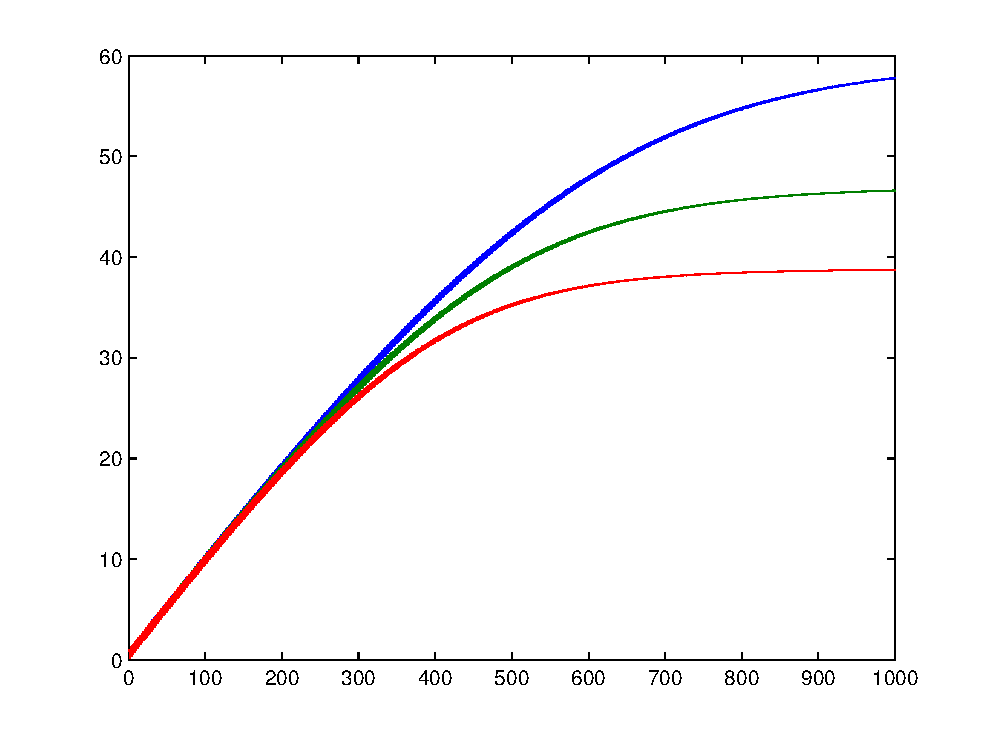
\includegraphics[width=0.4\textwidth]{simple.pdf} 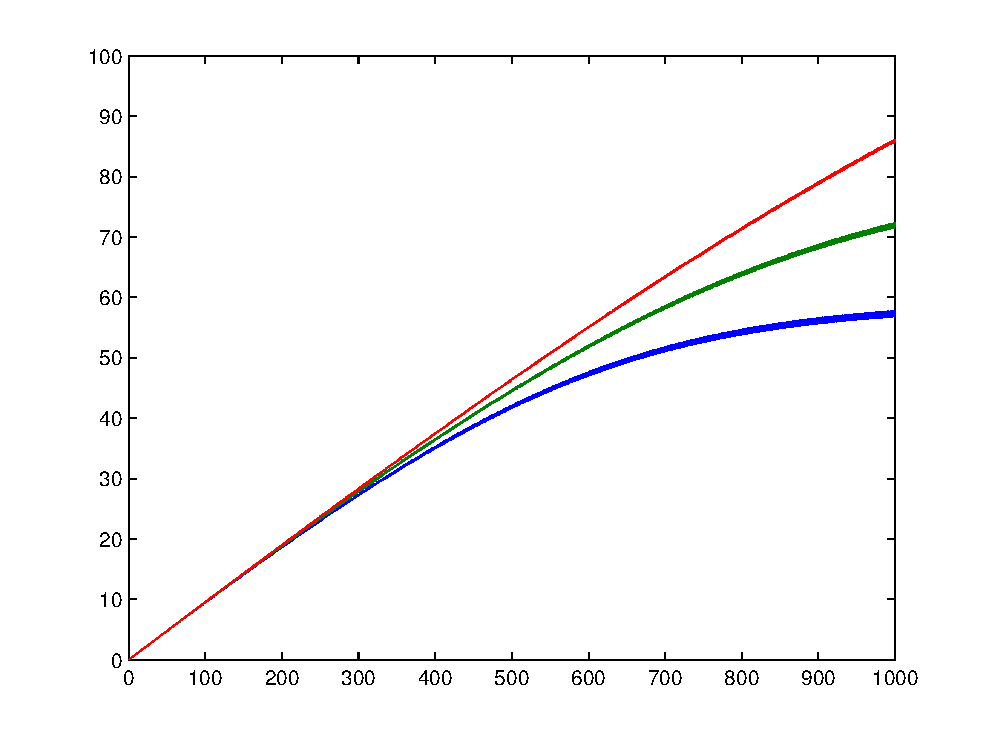
\includegraphics[width=0.4\textwidth]{tricky.pdf}
        \end{center}
        \caption{Regret as a function of time for exponentiated gradient (blue), multiplicative updates (green), and adaptive exponentiated gradient (red). Left: 
        the suboptimal strategies have high variance and the optimal strategy has low variance. Right: the suboptimal strategies have low variance and the 
        optimal strategy has high variance.}
        \label{fig:simple}
\end{figure}

\section{General Algorithms and Theoretical Analysis}

\begin{table}
\begin{tabular}{|c|c|c|} \hline
        Algorithm & Regret \\ \hline
        Exponentiated gradient & $\frac{\lambda n + \sum_{i=1}^n w_i[\log(w_i/\lambda)-1]}{\eta} + \eta \sum_{t=1}^T \sum_{i=1}^n w_{t,i}z_{t,i}^2$ \\ \hline
        Multiplicative updates & $\frac{\lambda n + \sum_{i=1}^n w_i[\log(w_i/\lambda)-1]}{\eta} + \eta \sum_{t=1}^T \sum_{i=1}^n w_{i}z_{t,i}^2$ \\ \hline
        Adaptive exponentiated gradient & $\frac{\lambda n + \sum_{i=1}^n w_i[\log(w_i/\lambda)-1]}{\eta} + \eta \sum_{t=1}^T \sum_{i=1}^n w_iz_{t,i}^2$ \\ \hline
\end{tabular}
\caption{Comparison of exponentiated gradient, multiplicative updates, and adaptive exponentiated gradient algorithms in the unconstrained case.}
\label{fig:unconstrained}
\end{table}

We now present the unconstrained versions of our three algorithms, together 
with an analysis based on adaptive regularizers (the bounds can be found summarized 
in Table~\ref{fig:unconstrained}). In each case, the weight 
vector $w$ is necessarily non-negative. We can deal with this constraint by 
maintaining two weight vectors $w_+$ and $w_-$ and predicting with $w_+-w_-$ 
(this is a standard idea, going back at least to the original exponentiated 
gradient paper by Kivinen and Warmuth). This is equivalent to replacing the 
gradient $z$ with the expanded vector $\left[ \begin{array}{cc} z \\ -z \end{array} \right]$. 
For simplicity of exposition, we will simply assume that $w$ is constrained 
to be non-negative in our algorithms and analysis.

Each algorithm can be interpreted as (adaptive) mirror descent with an appropriate 
regularizer. Each regularizer will (potentially) vary with the round $t$, and will be a 
member of the family $\psi_u(w)$, which for $u \in \bR^n$ is defined as
\[ \psi_u(w) \eqdef \sum_{i=1}^n w_i[\log(w_i/\lambda)-1] + u^{\top}w. \]
The parameter $\lambda$ is a hyperparameter controlling the size of $w$. Typically it should be on the order of $\frac{1}{n}$ 
(as we will see more explicitly when we prove a formal regret bound). 
Before continuing, it will be useful to point out a few properties of $\psi_u$, which we 
state in Lemma~\ref{lem:properties} and prove in the Appendix.
\begin{lemma}
\label{lem:properties}
For $\psi_u(w) \eqdef \sum_{i=1}^n w_i[\log(w_i/\lambda)-1] + u^{\top}w$, we have:
\begin{align}
\psi_u^*(\theta) &= \lambda \sum_{i=1}^n \exp(\theta_i - u_i). \\
\frac{\partial \psi_i^*}{\partial \theta_i} &= \lambda \exp(\theta_i - u_i). 
\end{align}
\end{lemma}
Now, as noted above, each of the three algorithms can be expressed in terms of a 
time-varying regularizer $\psi_t(w) \equiv \psi_{u_t}(w)$. The particular choices of $u_t$ are:
\begin{enumerate}
        \item \textbf{Exponentiated gradient:} $u_{t,i} = 0$ (non-varying regularizer) %$\psi_t(w) = \sum_{i=1}^n w_i[\log(w_i/\lambda)-1]$.
        \item \textbf{Multiplicative updates:} $u_{t,i} = -\sum_{s=1}^t \eta z_{s,i} + \log(1-\eta z_{s,i})$ %$\psi_t(w) = \sum_{i=1}^n w_i[\log(w_i/\lambda)-1-\sum_{s=1}^t (\eta z_{s,i} + \log(1-\eta z_{s,i}))]$.
        \item \textbf{Adaptive exponentiated gradient:} $u_{t,i} = \eta \sum_{s=1}^t z_{s,i}^2$ %$\psi_t(w) = \sum_{i=1}^n w_i[\log(w_i/\lambda)-1+\sum_{s=1}^t \eta^2 z_{s,i}^2 w_i]$.
\end{enumerate}
Note that in the limit of small $\eta$, 
$-\eta z_{t,i} - \log(1-\eta z_{t,i}) \approx \frac{1}{2}\eta z_{t,i}^2$, so that 
the latter two regularizers are in fact very similar. The mirror descent updates corresponding 
to each of the above regularizers are:
\begin{enumerate}
        \item \textbf{Exponentiated gradient:} $w_{t,i} = \lambda \cdot \exp\left(-\eta \sum_{t=1}^T z_{t,i}\right)$
        \item \textbf{Multiplicative updates:} $w_{t,i} = \lambda \cdot \prod_{t=1}^T (1- \eta z_{t,i})$
        \item \textbf{Adaptive exponentiated gradient:} $w_{t,i} = \lambda \cdot \exp\left(- \sum_{t=1}^T \eta z_{t,i} + \eta^2 z_{t,i}^2\right)$
\end{enumerate}
Finally, we base our regret bounds on an adaptation of the mirror descent analysis. In the analysis of 
mirror descent based on Fenchel conjugacy, we have the following inequality for any regularizer $\psi$; 
letting $\theta_t \eqdef -\sum_{s=1}^T z_s$ and $\psi_t$ denote the regularizer at time $t$:
\begin{equation}
        \label{eqn:bound1}
        -\psi_T(w) - \eta \sum_{t=1}^T w^{\top} z_t \leq \psi_0^*(0) + \sum_{t=1}^T \psi_t^*(\theta_t) - \psi_{t-1}^*(\theta_{t-1}).
\end{equation}
Usually the regularizer is fixed, in which case $\psi^*(\theta_t) - \psi^*(\theta_{t-1}) = -\eta w_t^{\top}z_t + D_{\psi^*}(\theta_{t+1} \| \theta_t)$. 
Note that $w_t^{\top}z_t$ is the loss suffered in round $t$; the Bregman divergence term $D_{\psi^*}$ measures the increase in regret for that round. 
In particular, re-arranging gives
\begin{equation}
        \label{eqn:bound2}
        \Regret(w) = \sum_{t=1}^T w_t^{\top}z_t - \sum_{t=1}^T w^{\top}z_t \leq \frac{1}{\eta}\left[ \psi^*(0) + \psi(w) + \sum_{t=1}^T D_{\psi^*}(\theta_{t+1} \| \theta_t)\right].
\end{equation}
One can then use an analysis based on strong convexity of $\psi$ to bound $\psi^*$; for instance, in the case of exponentiated gradient, 
we have the bound $D_{\psi^*}(\theta_{t+1} \| \theta_t) \leq \eta^2 \sum_{i=1}^n w_{t,i}z_{t,i}^2$, which leads to our claimed regret bound 
for exponentiated gradient.

In contrast, our analysis based on adaptive regularizers will choose $\psi_t^*$ such that $\psi_t^*(\theta_t) - \psi_{t-1}^*(\theta_{t-1}) \leq -\eta w_t^{\top}z_t$. 
Assuming we succeed in picking such a $\psi_t^*$, the $\sum_{t=1}^T \psi_t^*(\theta_t) - \psi_{t-1}^*(\theta_{t-1})$ term can be replaced with 
$-\eta \sum_{t=1}^T w_t^{\top}z_t$. We can then re-arrange to obtain the regret bound
\begin{equation}
        \label{eqn:bound3}
        \Regret(w) = \sum_{t=1}^T w_t^{\top}z_t - \sum_{t=1}^T w^{\top}z_t \leq \frac{\psi_0^*(0) + \psi_T(w)}{\eta}.
\end{equation}
This is quite interesting as we have pushed the entire regret bound into an increase in the size 
of the regularizer.

We will now verify the property $\psi_t^*(\theta_t) - \psi_{t-1}^*(\theta_{t-1}) \leq -\eta w_t^{\top}z_t$ 
for both multiplicative updates and adaptive EG. Our analysis relies on Lemma~\ref{lem:properties}.
For multiplicative updates:
\begin{align}
        \psi_t^*(\theta_t) &= \psi_t^*(\theta_{t-1}- \eta z_t) \\
                           &= \lambda \sum_{i=1}^n \exp\left(\theta_{t-1,i} - \eta z_{t,i} - u_{t,i}\right) \\
                           &= \lambda \sum_{i=1}^n \exp\left(\theta_{t-1,i} + \log(1- \eta z_{t,i}) - u_{t-1,i}\right) \\
                           &= \lambda \sum_{i=1}^n \exp\left(\theta_{t-1,i} - u_{t-1,i}\right)(1 - \eta z_{t,i}) \\
                           &= \psi_{t-1}^*(\theta_{t-1}) - \eta \lambda \sum_{i=1}^n \exp\left(\theta_{t-1,i} - u_{t-1,i}\right) z_{t,i} \\
                           &= \psi_{t-1}^*(\theta_{t-1}) - \eta w_t^{\top}z_t,
\end{align}
hence $\psi_t^*(\theta_t) - \psi_{t-1}^*(\theta_{t-1}) = -\eta w_t^{\top}z_t$, i.e. the property holds with equality. Using the 
fact that $\eta z + \log(1-\eta z) \leq \eta^2 z^2$ for $\eta \leq \frac{1}{2z}$, we have the regret bound
\begin{align}
        \Regret(w) &\leq \frac{\psi_0*(0) + \psi_T(w)}{\eta} \\
                   &= \frac{\lambda n + \sum_{i=1}^n w_i[\log(w_i/\lambda)-1] + u_T^{\top}w}{\eta} \\
                   &\leq \frac{\lambda n + \sum_{i=1}^n w_i[\log(w_i/\lambda)-1] + \eta^2 \sum_{i=1}^n w_i \sum_{t=1}^T z_{t,i}^2}{\eta} \\
                   &= \frac{\lambda n + \sum_{i=1}^n w_i[\log(w_i/\lambda)-1]}{\eta} + \eta \sum_{t=1}^T \sum_{i=1}^n w_i z_{t,i}^2,
\end{align}
which holds whenever $\eta \leq \frac{1}{2 \max_{t=1}^T \|z_t\|_{\infty}}$. 

Setting $\lambda$ to $1/n$ yields a bound of
\[ \Regret(w) \leq \frac{1+(\log(n)-1)\|w\|_1 + \sum_{i=1}^n w_i\log(w_i)}{\eta} + \eta \sum_{t=1}^T \sum_{i=1}^n w_i z_{t,i}^2. \]
The proof for adaptive exponentiated gradient is similar; we have:
\begin{align}
\psi_t^*(\theta_t) &= \psi_t^*(\theta_{t-1} - \eta z_t) \\
 &= \lambda \sum_{i=1}^n \exp\left(\theta_{t-1,i} - \eta z_{t,i} - u_{t,i}\right) \\
 &= \lambda \sum_{i=1}^n \exp\left(\theta_{t-1,i} - \eta z_{t,i} - \eta^2 z_{t,i}^2 - u_{t-1,i}\right) \\
 &= \lambda \sum_{i=1}^n \exp\left(\theta_{t-1,i} - u_{t-1,i}\right)\exp(-\eta z_{t,i} - \eta^2 z_{t,i}^2) \\
 &\leq \lambda \sum_{i=1}^n \exp\left(\theta_{t-1,i} - u_{t-1,i}\right)(1-\eta z_{t,i}) \\
 &= \psi_{t-1}^*(\theta_{t-1}) - \eta w_t^{\top}z_t,
\end{align}
where the last step re-uses the analysis for multiplicative updates. We thus have
\begin{align}
\Regret(w) &\leq \frac{\psi_0^*(0) + \psi_T(w)}{\eta} \\
 &= \frac{\lambda n + \sum_{i=1}^n w_i[\log(w_i/\lambda)-1]}{\eta} + \eta \sum_{t=1}^T \sum_{i=1}^n w_i z_{t,i}^2,
\end{align}
which is the same regret bound as before.
\section{Experiments}
TODO.

\end{document}
